\documentclass[11pt,a4paper]{article}

\usepackage[utf8]{inputenc}
\usepackage[T1]{fontenc}
\usepackage[italian]{babel}
\usepackage{geometry}
\usepackage{graphicx}
\usepackage[table]{xcolor}
\usepackage{hyperref}
\usepackage{booktabs}
\usepackage{longtable}
\usepackage{array}
\usepackage{float}
\usepackage{caption}
\usepackage{fancyhdr}
\usepackage{tikz}
\usepackage{listings}

\usetikzlibrary{arrows.meta,positioning,fit,shapes.geometric,calc}

\geometry{margin=2.3cm}
\graphicspath{{figures/}}
\hypersetup{
  colorlinks=true,
  linkcolor=blue!55!black,
  urlcolor=blue!55!black,
  citecolor=blue!55!black,
  pdftitle={ParcheggIA - Relazione tecnica},
  pdfauthor={Alberto Bocchieri}
}

\definecolor{pgDark}{HTML}{061018}
\definecolor{pgBlue}{HTML}{2F80FF}
\definecolor{pgGreen}{HTML}{35C56A}
\definecolor{pgYellow}{HTML}{F2C94C}
\definecolor{pgRed}{HTML}{EB5757}
\definecolor{pgPanel}{HTML}{F4F7FB}
\definecolor{pgLine}{HTML}{C7D0DD}

\pagestyle{fancy}
\setlength{\headheight}{14pt}
\fancyhf{}
\lhead{ParcheggIA}
\rhead{Relazione tecnica}
\cfoot{\thepage}

\captionsetup{font=small, labelfont=bf}
\renewcommand{\arraystretch}{1.18}

\lstdefinestyle{pgcode}{
  basicstyle=\ttfamily\small,
  breaklines=true,
  frame=single,
  rulecolor=\color{pgLine},
  backgroundcolor=\color{pgPanel},
  keywordstyle=\color{pgBlue},
  commentstyle=\color{gray!70!black}
}
\lstset{style=pgcode}

\newcommand{\service}[1]{\texttt{#1}}
\newcommand{\api}[1]{\texttt{#1}}

\begin{document}

\begin{titlepage}
  \centering
  \vspace*{1.6cm}
  {\Huge\bfseries ParcheggIA\par}
  \vspace{0.35cm}
  {\Large Relazione tecnica del progetto di Sistemi Cloud\par}
  \vspace{1.2cm}
  \begin{tikzpicture}
    \node[
      rounded corners=18pt,
      fill=pgDark,
      minimum width=0.86\textwidth,
      minimum height=6.0cm,
      text width=0.72\textwidth,
      align=center,
      inner sep=20pt
    ] (box) {};
    \node[font=\bfseries\Huge, text=white] at ($(box.center)+(0,1.25)$) {ParcheggIA};
    \node[font=\Large, text=white!82, text width=0.62\textwidth, align=center] at ($(box.center)+(0,0.35)$)
      {Stima predittiva della disponibilit\`a di parcheggio su segmenti stradali reali};
    \draw[line width=9pt, rounded corners=20pt, pgGreen] ($(box.center)+(-4.3,-1.4)$) -- ++(2.4,0.55) -- ++(2.0,-0.35);
    \draw[line width=9pt, rounded corners=20pt, pgYellow] ($(box.center)+(-0.4,-1.15)$) -- ++(2.4,0.45) -- ++(2.2,-0.65);
    \draw[line width=9pt, rounded corners=20pt, pgRed] ($(box.center)+(-3.4,-2.15)$) -- ++(3.1,0.15) -- ++(3.6,-0.2);
    \node[circle, fill=pgBlue, draw=white, line width=2pt, minimum size=0.86cm] at ($(box.center)+(0,-1.35)$) {};
    \node[regular polygon, regular polygon sides=3, fill=white, minimum size=0.42cm, rotate=0] at ($(box.center)+(0,-1.30)$) {};
  \end{tikzpicture}
  \vfill
  {\large Alberto Bocchieri\par}
  \vspace{0.2cm}
  {\large \today\par}
\end{titlepage}

\tableofcontents
\newpage

\section{Introduzione}

ParcheggIA nasce come progetto cloud-native con un obiettivo pratico: aiutare un automobilista a capire dove conviene cercare parcheggio nelle immediate vicinanze, evitando sia una mappa generica sia un semplice elenco statico di aree. La scelta progettuale principale \`e stata quindi spostare il centro del sistema dal concetto ampio di ``zona'' al concetto pi\`u fine di segmento stradale. Ogni tratto di strada \`e analizzato come unit\`a indipendente, con un nome via, una geometria, un tipo di sosta e una percentuale stimata di probabilit\`a di trovare posto.

Il risultato \`e una demo che combina tre aspetti normalmente separati:

\begin{itemize}
  \item una interfaccia di guida in stile navigatore, costruita con MapLibre GL JS e pensata per essere usata a colpo d'occhio;
  \item una pipeline dati che parte da OpenStreetMap, integra override locali sulle strisce blu e aggiorna le stime attraverso report, segnali simulati o dati TomTom;
  \item una architettura a microservizi, eseguibile in locale con Docker Compose, simulabile su Kubernetes locale con k3d e distribuibile su AWS con servizi gestiti.
\end{itemize}

Il progetto \`e stato pensato anche per essere dimostrabile senza chiavi esterne. In assenza di TomTom, Nemotron ed ElevenLabs, la piattaforma continua a funzionare con dati OSM reali, predizioni simulate, suggerimenti AI simulati e Text-to-Speech del browser. Le integrazioni reali sono abilitate solo quando vengono fornite le relative API key, senza mai esporle nel frontend.

\section{Obiettivi e requisiti}

Dal punto di vista funzionale, ParcheggIA deve rispondere a una domanda semplice: ``se mi trovo qui, in quale strada vicina ha pi\`u senso cercare parcheggio?''. Per rendere credibile la risposta, il sistema non pu\`o limitarsi a colorare grandi quartieri. Deve invece lavorare con segmenti piccoli, preferibilmente identificabili con il nome della via, e deve distinguere tra strisce blu, sosta probabilmente libera, sosta limitata o informazioni non note.

Dal punto di vista architetturale, il progetto deve mostrare competenze di Sistemi Cloud. Per questo la stessa applicazione \`e stata sviluppata in tre modalit\`a operative:

\begin{enumerate}
  \item \textbf{locale}, con Docker Compose, adatta allo sviluppo e alla correzione rapida;
  \item \textbf{Kubernetes locale}, con k3d, per simulare l'organizzazione cloud senza costi;
  \item \textbf{AWS reale}, con EKS, RDS, ElastiCache, Amazon MQ, ECR, Terraform, SSM e script di accensione e spegnimento.
\end{enumerate}

Queste tre modalit\`a non sono tre applicazioni diverse. Sono tre modi di avviare lo stesso sistema, con lo stesso frontend, gli stessi microservizi e gli stessi contratti API. Cambiano invece i componenti infrastrutturali sottostanti: in locale PostgreSQL, Redis e RabbitMQ sono container; su AWS diventano servizi gestiti.

\section{Esperienza utente}

La GUI \`e stata progettata come interfaccia di guida, non come dashboard amministrativa. Questo ha portato a una serie di scelte concrete: mappa full-screen, pannelli grandi, pochi testi, controlli laterali, dock inferiore, marker leggibili e suggerimenti vocali. L'utente deve poter capire rapidamente se un tratto \`e favorevole, incerto o critico.

\begin{figure}[H]
  \centering
  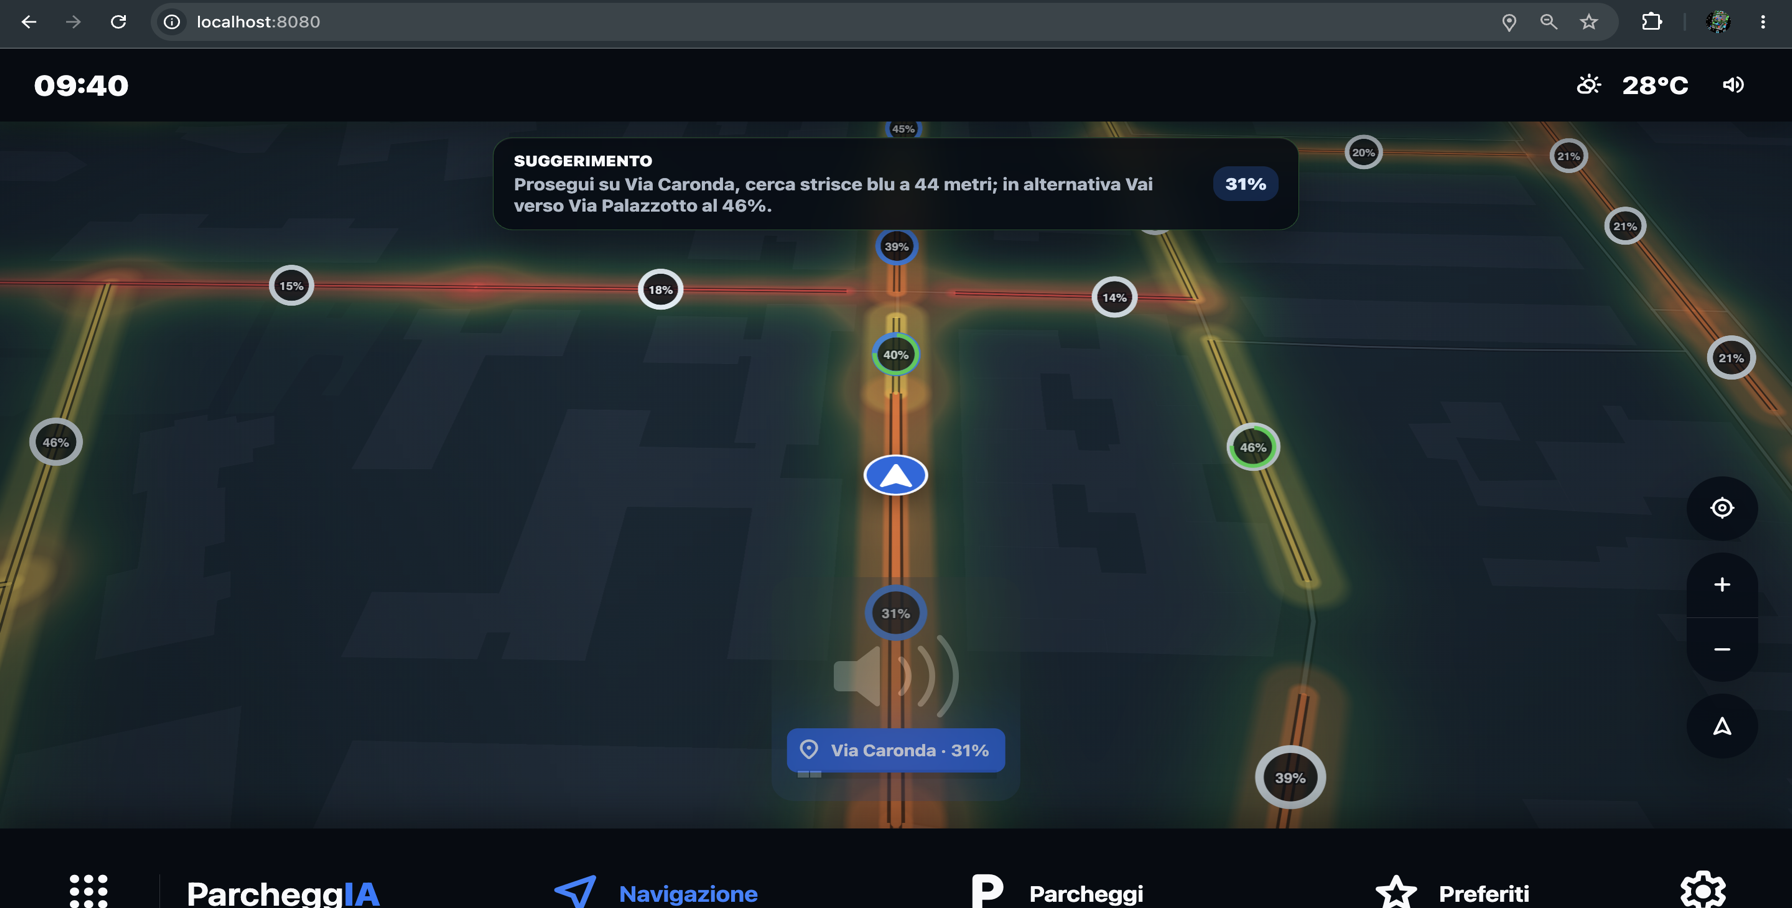
\includegraphics[width=\textwidth]{screenshot_app_main.png}
  \caption{Schermata reale della GUI locale: mappa scura, heatmap continua sui segmenti, marker percentuali, suggerimento AI e controlli stile navigatore.}
  \label{fig:gui}
\end{figure}

\begin{figure}[H]
  \centering
  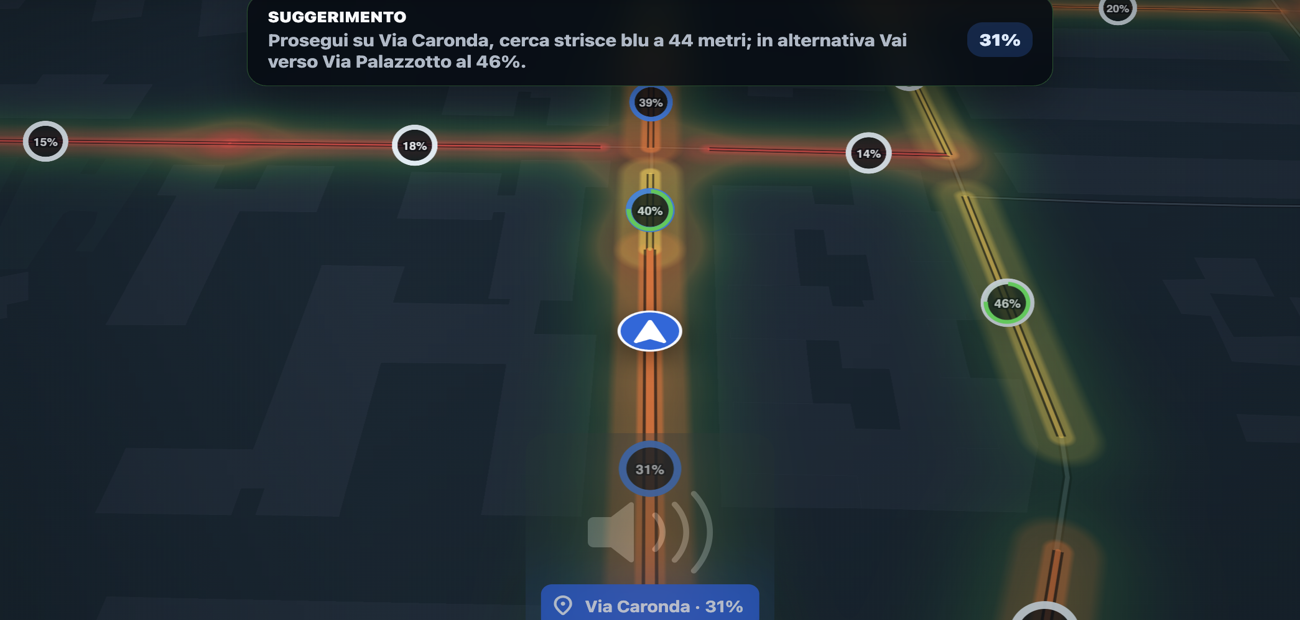
\includegraphics[width=0.92\textwidth]{screenshot_app_detail.png}
  \caption{Dettaglio della visuale di guida: il suggerimento operativo, la posizione utente orientata e i marker di disponibilit\`a restano leggibili senza coprire la mappa.}
  \label{fig:gui-detail}
\end{figure}

La mappa \`e basata su MapLibre GL JS. Questa scelta \`e stata preferita a Leaflet perch\'e MapLibre lavora nativamente con WebGL, supporta pitch e bearing, gestisce meglio layer vettoriali, heatmap, linee continue e marker sovrapposti. Per una interfaccia di guida, la capacit\`a di inclinare la camera e orientarla nel senso di marcia \`e fondamentale.

Le informazioni principali mostrate a schermo sono:

\begin{itemize}
  \item heatmap continua lungo le strade, con colori che indicano la difficolt\`a stimata;
  \item marker sui segmenti, con bordo colorato in base al tipo di sosta e percentuale al centro;
  \item marker dei parcheggi individuati tramite Search API o fallback simulato;
  \item chip centrale con strada corrente e percentuale;
  \item suggerimento AI a comparsa dall'alto, letto anche tramite TTS quando disponibile;
  \item simulazione guida da 500 metri per mostrare il comportamento dinamico senza dover usare un'auto reale.
\end{itemize}

\subsection{Percentuali e colori}

La percentuale rappresenta una stima di \emph{parkability}, cio\`e la probabilit\`a pratica di trovare posto. Non \`e una misura legale e non sostituisce la segnaletica sul posto. Le soglie usate nella GUI sono volutamente semplici:

\begin{center}
\begin{tabular}{@{}llc@{}}
\toprule
Intervallo & Interpretazione & Colore prevalente \\
\midrule
$<20\%$ & molto difficile & rosso \\
$20$--$39\%$ & difficile & rosso/arancio \\
$40$--$59\%$ & incerto & giallo \\
$60$--$79\%$ & buono & verde \\
$\geq80\%$ & favorevole & verde intenso \\
\bottomrule
\end{tabular}
\end{center}

La heatmap non \`e generata con punti isolati. Ogni segmento viene campionato lungo la sua geometria e poi visualizzato con un layer morbido e ribbon lineari sovrapposti. Questo evita l'effetto ``pallini'' e rende la disponibilit\`a visivamente continua lungo la strada.

\section{Architettura generale}

L'architettura segue un modello a microservizi. Il frontend comunica solo con l'API Gateway; nessuna API key esterna viene mai inviata al browser. I servizi interni si dividono le responsabilit\`a: dati geografici, predizione, sessione utente, ingestion di eventi, amministrazione e AI.

\begin{figure}[H]
\centering
\resizebox{\textwidth}{!}{%
\begin{tikzpicture}[
  node distance=0.9cm and 1.1cm,
  box/.style={draw=pgLine, rounded corners=4pt, fill=white, align=center, minimum height=0.8cm, text width=2.8cm},
  store/.style={draw=pgLine, cylinder, shape border rotate=90, aspect=0.22, fill=pgPanel, align=center, minimum height=1.0cm, text width=2.5cm},
  ext/.style={draw=pgBlue, rounded corners=4pt, fill=blue!5, align=center, minimum height=0.8cm, text width=2.6cm},
  arr/.style={-{Latex[length=2.5mm]}, thick, color=gray!70!black}
]
  \node[ext] (browser) {Browser\\MapLibre};
  \node[box, right=of browser] (gateway) {API Gateway\\Nginx};
  \node[box, right=of gateway, yshift=1.5cm] (zone) {Zone Service\\segmenti e strade};
  \node[box, right=of gateway, yshift=0.45cm] (pred) {Prediction\\Service};
  \node[box, right=of gateway, yshift=-0.60cm] (loc) {Location\\Service};
  \node[box, right=of gateway, yshift=-1.65cm] (ai) {Nemotron\\Service};
  \node[box, below=1.0cm of pred] (ing) {Ingestion\\Service};
  \node[box, below=1.0cm of loc] (admin) {Admin\\Service};

  \node[store, right=1.4cm of zone] (pg) {PostgreSQL\\PostGIS};
  \node[store, right=1.4cm of pred] (redis) {Redis};
  \node[store, right=1.4cm of ing] (rabbit) {RabbitMQ};
  \node[ext, right=1.2cm of redis] (external) {TomTom\\Nemotron\\ElevenLabs};

  \draw[arr] (browser) -- (gateway);
  \draw[arr] (gateway) -- (zone);
  \draw[arr] (gateway) -- (pred);
  \draw[arr] (gateway) -- (loc);
  \draw[arr] (gateway) -- (ai);
  \draw[arr] (gateway) |- (ing);
  \draw[arr] (gateway) |- (admin);

  \draw[arr] (zone) -- (pg);
  \draw[arr] (pred) -- (pg);
  \draw[arr] (pred) -- (redis);
  \draw[arr] (loc) -- (redis);
  \draw[arr] (ing) -- (redis);
  \draw[arr] (ing) -- (rabbit);
  \draw[arr] (rabbit) -- (zone);
  \draw[arr] (ing) -- (external);
  \draw[arr] (ai) -| (external);
\end{tikzpicture}
}
\caption{Vista logica dell'architettura a microservizi. Il frontend non parla mai direttamente con provider esterni.}
\label{fig:architecture}
\end{figure}

\subsection{Perch\'e microservizi}

Per una demo piccola si potrebbe implementare tutto in un unico backend. La scelta a microservizi \`e stata fatta perch\'e il requisito principale non \`e solo produrre una UI funzionante, ma mostrare una architettura cloud replicabile. Separare i servizi rende espliciti i confini:

\begin{itemize}
  \item il servizio geografico pu\`o evolvere indipendentemente dalla predizione;
  \item il servizio di ingestion pu\`o ricevere dati real-time senza bloccare le API utente;
  \item il servizio AI pu\`o essere spento o sostituito senza compromettere heatmap e navigazione;
  \item gateway, database, cache e broker hanno ruoli chiari anche quando vengono sostituiti da servizi AWS gestiti.
\end{itemize}

La controparte di questa scelta \`e una maggiore complessit\`a operativa. Per contenerla, la repo include script di avvio locale, simulazione Kubernetes, deploy cloud e spegnimento.

\section{Servizi applicativi}

\small
\begin{longtable}{@{}p{4.0cm}p{2.7cm}p{5.8cm}p{1.5cm}@{}}
\toprule
Servizio & Tecnologia & Responsabilit\`a & Porta locale \\
\midrule
\endhead
\service{frontend} & Nginx, HTML, CSS, JS, MapLibre & Interfaccia utente, mappa, heatmap, marker, simulazione guida, TTS browser & 8080 \\
\service{api-gateway} & Nginx & Reverse proxy unico per API interne e frontend & 8000 \\
\service{zone-service} & FastAPI, PostGIS & Segmenti OSM, rete stradale, nearest segment, heatmap e override sosta & 8001 \\
\service{prediction-service} & FastAPI, Redis, PostGIS & Calcolo percentuali, scoring, report, segnali TomTom/simulati & 8002 \\
\service{location-service} & FastAPI, Redis, RabbitMQ & Sessioni live, posizione corrente, orchestrazione dati vicini & 8003 \\
\service{ingestion-service} & FastAPI, Redis, RabbitMQ & Ingestion eventi, TomTom parsimonioso, budget e cache & 8004 \\
\service{nemotron-service} & FastAPI & Suggerimenti AI, fallback simulato, integrazione ElevenLabs TTS & 8005 \\
\service{admin-service} & FastAPI & Endpoint operativi e diagnostici & 8006 \\
\bottomrule
\end{longtable}
\normalsize

\section{Modello dati}

Il dato centrale \`e \service{parking\_segments}. Ogni riga rappresenta un piccolo tratto stradale, ricavato da OSM e diviso per incroci o lunghezza massima. A differenza delle vecchie zone demo, questi segmenti sono pensati per sovrapporsi alla rete stradale realmente visibile in MapLibre.

\begin{figure}[H]
\centering
\begin{tikzpicture}[
  entity/.style={draw=pgLine, rounded corners=4pt, fill=white, minimum width=3.9cm, minimum height=1.0cm, align=center},
  rel/.style={-{Latex[length=2.2mm]}, thick, color=gray!70!black}
]
  \node[entity] (segments) {\textbf{parking\_segments}\\id, street\_name, geometry\\parking\_type, confidence};
  \node[entity, right=1.6cm of segments] (edges) {\textbf{road\_edges}\\geometry, source\\rete navigabile};
  \node[entity, above=1.1cm of edges] (nodes) {\textbf{road\_nodes}\\intersezioni};
  \node[entity, below=1.1cm of edges] (lots) {\textbf{parking\_lots}\\POI parcheggio\\coordinate, indirizzo};
  \node[entity, below=1.1cm of segments] (reports) {\textbf{segment\_reports}\\tipo report\\timestamp, peso};
  \node[entity, left=1.5cm of reports] (redis) {\textbf{Redis keys}\\segment:signals:*\\sessioni live};

  \draw[rel] (nodes) -- (edges);
  \draw[rel] (edges) -- (segments);
  \draw[rel] (lots) -- (segments);
  \draw[rel] (reports) -- (segments);
  \draw[rel] (reports) -- (redis);
  \draw[rel] (redis) -- (segments);
\end{tikzpicture}
\caption{Modello dati semplificato: segmenti per la sosta, rete stradale per la navigazione, Redis per segnali dinamici.}
\label{fig:data-model}
\end{figure}

\subsection{Import OSM e override}

La pipeline offline importa la rete stradale di Catania da OpenStreetMap. I segmenti vengono puliti, spezzati e caricati in PostgreSQL/PostGIS. Successivamente vengono applicati override locali per rappresentare meglio strisce blu, limitazioni e aree note. Questa distinzione \`e importante: OSM fornisce la geometria stradale, mentre gli override correggono informazioni specifiche sulla sosta che spesso non sono complete nei dati aperti.

Il flusso offline \`e:

\begin{center}
\resizebox{\textwidth}{!}{%
\begin{tikzpicture}[
  flowstep/.style={draw=pgLine, rounded corners=4pt, fill=pgPanel, align=center, minimum height=0.9cm, text width=3.1cm},
  arr/.style={-{Latex[length=2.4mm]}, thick, color=gray!70!black}
]
  \node[flowstep] (osm) {OSM Catania\\strade e geometrie};
  \node[flowstep, right=of osm] (split) {Script import\\split per incroci\\e max 120 m};
  \node[flowstep, right=of split] (sql) {SQL dati\\catania\_segments};
  \node[flowstep, right=of sql] (pg) {PostGIS\\parking\_segments\\road\_edges};
  \node[flowstep, below=0.8cm of sql] (over) {Override\\strisce blu\\tariffe e fonti};
  \draw[arr] (osm) -- (split);
  \draw[arr] (split) -- (sql);
  \draw[arr] (sql) -- (pg);
  \draw[arr] (over) -- (pg);
\end{tikzpicture}
}
\end{center}

\section{Predizione}

La predizione non pretende di essere un modello statistico completo. In questa fase \`e un modello rule-based spiegabile, costruito per essere leggibile e integrabile con fonti real-time. Il punteggio parte da una baseline legata al tipo di sosta e viene corretto da segnali dinamici.

\begin{center}
\begin{tabular}{@{}lcc@{}}
\toprule
Tipo sosta & Baseline disponibilit\`a & Confidence iniziale \\
\midrule
Strisce blu & 42\% & 70\% \\
Probabile libero & 48\% & 52\% \\
Limitato & 14\% & 66\% \\
Ignoto & 42\% & 42\% \\
\bottomrule
\end{tabular}
\end{center}

Le correzioni principali sono:

\begin{itemize}
  \item report recenti degli utenti, con effetto positivo o negativo sul segmento corrente e sui segmenti vicini;
  \item segnali TomTom o simulati, salvati su Redis come pressione traffico e pressione evento;
  \item ora e giorno, perch\'e la disponibilit\`a cambia nelle ore trafficate, di notte e nel weekend;
  \item distanza dal punto utente, per dare pi\`u peso ai segmenti immediatamente vicini.
\end{itemize}

\begin{figure}[H]
\centering
\begin{tikzpicture}[x=2.4cm,y=0.065cm]
  \draw[->, color=gray!70] (0,0) -- (0,82) node[above, font=\scriptsize] {\%};
  \draw[->, color=gray!70] (0,0) -- (5.0,0);
  \foreach \y in {20,40,60,80} {
    \draw[color=pgLine] (0,\y) -- (4.75,\y);
    \node[left, font=\scriptsize] at (0,\y) {\y};
  }
  \draw[fill=pgBlue!75, draw=pgBlue!90!black] (0.45,0) rectangle (0.95,42);
  \node[above, font=\scriptsize\bfseries] at (0.7,42) {42\%};
  \node[below, font=\scriptsize] at (0.7,-3) {Blu};

  \draw[fill=pgGreen!75, draw=pgGreen!90!black] (1.55,0) rectangle (2.05,48);
  \node[above, font=\scriptsize\bfseries] at (1.8,48) {48\%};
  \node[below, font=\scriptsize, align=center] at (1.8,-3) {Libero prob.};

  \draw[fill=pgRed!75, draw=pgRed!90!black] (2.65,0) rectangle (3.15,14);
  \node[above, font=\scriptsize\bfseries] at (2.9,14) {14\%};
  \node[below, font=\scriptsize] at (2.9,-3) {Limitato};

  \draw[fill=pgYellow!75, draw=pgYellow!90!black] (3.75,0) rectangle (4.25,42);
  \node[above, font=\scriptsize\bfseries] at (4.0,42) {42\%};
  \node[below, font=\scriptsize] at (4.0,-3) {Ignoto};
\end{tikzpicture}
\caption{Baseline usate dal modello predittivo prima dei segnali dinamici.}
\label{fig:baseline}
\end{figure}

\subsection{Uso parsimonioso di TomTom}

TomTom viene usato solo backend-side. La GUI chiama endpoint interni; il servizio di ingestion decide se usare cache o fare una chiamata reale. La strategia \`e volutamente conservativa:

\begin{itemize}
  \item raggio operativo di circa 500 metri intorno all'utente;
  \item cella di cache di circa 250 metri;
  \item TTL minimo di 5 minuti;
  \item nessuna chiamata a TomTom per singolo segmento;
  \item budget guard in Redis per evitare consumo eccessivo.
\end{itemize}

In pratica una nuova zona live pu\`o consumare fino a poche chiamate Traffic Flow e una chiamata Traffic Incidents; muoversi dentro la stessa cella non consuma nuove quote. Questo \`e coerente con l'uso previsto: aggiornare il contesto locale, non interrogare il provider a ogni movimento sulla mappa.

\section{Flusso end-to-end}

Il seguente esempio mostra il percorso di un dato dalla sua origine fino alla visualizzazione. Si considera il caso in cui l'utente clicchi su una strada o venga spostato dalla simulazione guida.

\begin{figure}[H]
\centering
\begin{tikzpicture}[
  actor/.style={draw=pgBlue, rounded corners=4pt, fill=blue!5, align=center, minimum width=2.8cm, minimum height=0.8cm},
  svc/.style={draw=pgLine, rounded corners=4pt, fill=white, align=center, minimum width=2.8cm, minimum height=0.8cm},
  store/.style={draw=pgLine, rounded corners=4pt, fill=pgPanel, align=center, minimum width=2.8cm, minimum height=0.8cm},
  arr/.style={-{Latex[length=2.3mm]}, thick, color=gray!70!black}
]
  \node[actor] (ui) {Browser\\MapLibre};
  \node[svc, right=0.8cm of ui] (gw) {API Gateway};
  \node[svc, right=0.8cm of gw, yshift=1.0cm] (zone) {Zone Service};
  \node[svc, right=0.8cm of gw] (loc) {Location Service};
  \node[svc, right=0.8cm of gw, yshift=-1.0cm] (pred) {Prediction Service};
  \node[store, right=1.0cm of zone] (pg) {PostGIS};
  \node[store, right=1.0cm of pred] (redis) {Redis};
  \node[svc, below=0.9cm of loc] (ai) {Nemotron Service};

  \draw[arr] (ui) -- node[above, font=\scriptsize] {posizione} (gw);
  \draw[arr] (gw) -- (loc);
  \draw[arr] (loc) -- node[above, font=\scriptsize] {segmento corrente} (zone);
  \draw[arr] (zone) -- (pg);
  \draw[arr] (loc) -- node[below, font=\scriptsize] {prediction} (pred);
  \draw[arr] (pred) -- (redis);
  \draw[arr] (pred) -- (pg);
  \draw[arr] (loc) -- node[right, font=\scriptsize] {contesto} (ai);
  \draw[arr] (ai.west) -| node[below, font=\scriptsize] {suggerimento} (gw.south);
  \draw[arr] (gw) -- node[below, font=\scriptsize] {GeoJSON, chip, marker, AI} (ui);
\end{tikzpicture}
\caption{Flusso pratico: dalla posizione utente al rendering della mappa e al suggerimento AI.}
\label{fig:end-to-end}
\end{figure}

Nel dettaglio:

\begin{enumerate}
  \item il frontend aggiorna la posizione e la invia al gateway;
  \item il \service{location-service} aggiorna la sessione live in Redis;
  \item il \service{zone-service} cerca in PostGIS il segmento pi\`u vicino e i segmenti entro il raggio locale;
  \item il \service{prediction-service} calcola la percentuale combinando baseline, report, Redis e segnali dinamici;
  \item il frontend aggiorna heatmap, marker e chip centrale;
  \item quando serve, il \service{nemotron-service} genera un consiglio operativo usando il contesto disponibile;
  \item il TTS legge il suggerimento, usando ElevenLabs se configurato o il browser come fallback.
\end{enumerate}

\section{AI e Text-to-Speech}

Il servizio AI \`e separato dal resto del backend. Questo permette di tenere il sistema funzionante anche senza modello esterno e di non rallentare il calcolo delle predizioni. I suggerimenti non devono essere tecnici: l'utente non deve leggere termini come ``stima inferita'' o dettagli interni del modello. Il prompt chiede quindi consigli pratici, in italiano, basati solo sui segmenti e parcheggi presenti nel contesto.

Quando sono disponibili le chiavi:

\begin{itemize}
  \item Nemotron genera il suggerimento testuale;
  \item ElevenLabs genera una voce pi\`u naturale;
  \item la GUI mostra una card animata che scende dall'alto e si chiude quando il parlato termina.
\end{itemize}

Senza chiavi, il servizio restituisce una modalit\`a simulata, sufficiente per dimostrare il flusso end-to-end. La scelta \`e intenzionale: chi clona la repo deve vedere l'esperienza completa anche senza configurare provider esterni.

\section{Messaging, cache e asincronia}

Redis e RabbitMQ svolgono ruoli diversi. Redis \`e usato per stato breve, cache, sessioni live, budget e segnali predittivi. RabbitMQ \`e usato per eventi asincroni, ad esempio quando un report o una ingestion deve influenzare i segmenti senza bloccare la richiesta HTTP principale.

\begin{center}
\begin{tabular}{@{}lll@{}}
\toprule
Componente & Uso nel progetto & Alternativa cloud \\
\midrule
PostgreSQL/PostGIS & dati geografici persistenti & Amazon RDS PostgreSQL \\
Redis & cache, sessioni, segnali, budget & Amazon ElastiCache \\
RabbitMQ & eventi asincroni & Amazon MQ for RabbitMQ \\
Docker Registry & immagini locali o ECR & Amazon ECR \\
Kubernetes & orchestrazione container & Amazon EKS \\
\bottomrule
\end{tabular}
\end{center}

\section{Modalit\`a di esecuzione}

\subsection{Docker Compose}

Docker Compose \`e la modalit\`a di sviluppo pi\`u diretta. Un solo comando avvia database, cache, broker, microservizi e frontend:

\begin{lstlisting}[language=bash]
docker compose up -d --build
\end{lstlisting}

Il primo avvio pu\`o essere pi\`u lento perch\'e importa i segmenti OSM reali e applica gli override. Una volta completato, l'app \`e disponibile su \url{http://localhost:8080}. Questa modalit\`a \`e la pi\`u adatta per valutare la GUI e il comportamento base senza costi cloud.

\subsection{Kubernetes locale con k3d}

La simulazione cloud locale usa k3d per creare un cluster Kubernetes leggero sul PC. Lo scopo non \`e migliorare le prestazioni, ma mostrare la stessa forma operativa del cloud: pod, service, config, secret, import dati e port-forward.

\begin{lstlisting}[language=bash]
scripts/cloud_sim_local_up.sh
\end{lstlisting}

Questa modalit\`a \`e utile didatticamente perch\'e permette di vedere come l'app viene scomposta in workload Kubernetes senza pagare AWS. La differenza principale \`e che i servizi gestiti sono simulati da pod locali.

\subsection{AWS reale}

Il deploy AWS usa Terraform per creare l'infrastruttura e script shell per coordinare build, push immagini, configurazione Kubernetes e smoke test. La scelta dei servizi AWS rispecchia i requisiti del progetto:

\begin{itemize}
  \item \textbf{EKS} per eseguire i microservizi su Kubernetes gestito;
  \item \textbf{RDS PostgreSQL} per persistenza relazionale e PostGIS;
  \item \textbf{ElastiCache Redis} per cache e segnali;
  \item \textbf{Amazon MQ for RabbitMQ} per il broker gestito;
  \item \textbf{ECR} per conservare le immagini Docker;
  \item \textbf{SSM Parameter Store} per parametri e segreti applicativi;
  \item \textbf{Lambda/EventBridge} per programmare lo spegnimento automatico.
\end{itemize}

\begin{figure}[H]
\centering
\begin{tikzpicture}[
  node distance=0.7cm and 0.9cm,
  aws/.style={draw=orange!70!black, rounded corners=4pt, fill=orange!8, align=center, text width=2.7cm, minimum height=0.8cm},
  app/.style={draw=pgBlue, rounded corners=4pt, fill=blue!5, align=center, text width=2.7cm, minimum height=0.8cm},
  arr/.style={-{Latex[length=2.3mm]}, thick, color=gray!70!black}
]
  \node[aws] (lb) {Load Balancer};
  \node[aws, right=of lb] (eks) {EKS};
  \node[app, right=of eks, yshift=1.1cm] (pods) {Pod microservizi};
  \node[aws, right=of eks, yshift=0cm] (ecr) {ECR};
  \node[aws, right=of eks, yshift=-1.1cm] (ssm) {SSM};
  \node[aws, below=1.2cm of pods] (rds) {RDS};
  \node[aws, right=of rds] (cache) {ElastiCache};
  \node[aws, left=of rds] (mq) {Amazon MQ};
  \node[aws, below=1.0cm of eks] (lambda) {Lambda\\auto-down};

  \draw[arr] (lb) -- (eks);
  \draw[arr] (eks) -- (pods);
  \draw[arr] (ecr) -- (eks);
  \draw[arr] (ssm) -- (pods);
  \draw[arr] (pods) -- (rds);
  \draw[arr] (pods) -- (cache);
  \draw[arr] (pods) -- (mq);
  \draw[arr] (lambda) -- (eks);
\end{tikzpicture}
\caption{Mappatura cloud reale su AWS. Le risorse costose vengono spente con script e auto-down.}
\label{fig:aws}
\end{figure}

Poich\'e i servizi AWS hanno costo continuo, la demo cloud \`e stata pensata per essere accesa solo per periodi brevi. Gli script richiedono conferme esplicite e il comando di spegnimento elimina le risorse create. L'auto-spegnimento programmato a quattro ore riduce il rischio di lasciare l'ambiente acceso.

\section{Infrastructure as Code e CI/CD}

Terraform descrive l'infrastruttura cloud: VPC, EKS, RDS, Redis, RabbitMQ gestito, ECR, log group, SSM e funzioni di supporto. Questo rende l'ambiente riproducibile su un account AWS diverso, purch\'e l'utente abbia credenziali e quote adeguate. Ansible \`e presente come parte didattica dell'approccio IaC, ma il flusso principale \`e Terraform pi\`u script shell.

La CI/CD su GitHub Actions verifica il codice e costruisce immagini Docker. Una parte del lavoro \`e stata rendere le immagini pulite e pubblicabili su ECR, evitando dipendenze da file locali non presenti nel runner. Per il deploy cloud reale, la pipeline pu\`o essere estesa con credenziali AWS del repository, ma per sicurezza la demo resta controllabile anche da script locali.

\section{Sicurezza e gestione segreti}

Un vincolo importante \`e non esporre chiavi private. La regola adottata \`e:

\begin{itemize}
  \item nessuna chiave nel frontend;
  \item nessuna chiave committata nella repo;
  \item in locale, chiavi opzionali tramite \texttt{.env};
  \item in AWS, chiavi opzionali tramite SSM Parameter Store;
  \item fallback funzionanti quando le chiavi non sono disponibili.
\end{itemize}

Questo consente a chi clona il progetto di eseguirlo subito, ma permette anche una demo completa con provider reali quando l'ambiente \`e configurato.

\section{Testing e validazione}

Il progetto include controlli statici, smoke test e test end-to-end demo. I controlli non sostituiscono test di carico o validazione statistica del modello, ma verificano i contratti fondamentali:

\begin{itemize}
  \item il frontend contiene le integrazioni attese e non dipende da Leaflet;
  \item i servizi rispondono agli endpoint principali;
  \item i segmenti OSM sono importati;
  \item i contratti API sono coerenti;
  \item lo smoke test verifica gateway, dati, heatmap e path principali.
\end{itemize}

Comandi principali:

\begin{lstlisting}[language=bash]
scripts/static_checks.sh
scripts/smoke_test.sh
scripts/e2e_demo_test.sh
\end{lstlisting}

In cloud, gli script eseguono anche smoke test dopo il deploy, cos\`i il link pubblico viene restituito solo quando il frontend e le API risultano raggiungibili.

\section{Decisioni progettuali}

\subsection{MapLibre invece di Leaflet}

Leaflet \`e semplice e maturo, ma \`e pi\`u adatto a mappe 2D tradizionali. ParcheggIA richiede una visuale inclinata, layer lineari continui, marker numerosi e una sensazione di navigatore. MapLibre GL JS \`e quindi pi\`u adatto perch\'e usa WebGL e lavora bene con style vettoriali e trasformazioni camera.

\subsection{Segmenti OSM invece di grandi zone}

Le zone grandi sono facili da gestire, ma poco utili per un automobilista. Due strade adiacenti possono avere disponibilit\`a e regole di sosta molto diverse. I segmenti OSM permettono consigli pi\`u concreti: ``prosegui su Via Caronda'' \`e molto pi\`u utile di ``zona centro''.

\subsection{Fallback simulati}

Il fallback non \`e un ripiego marginale, ma una scelta di prodotto e di valutazione. Un progetto didattico deve poter essere avviato da chiunque senza account TomTom, NVIDIA o ElevenLabs. I fallback permettono di verificare architettura, GUI e flussi anche in ambienti isolati.

\subsection{AWS gestito}

EKS, RDS, ElastiCache e Amazon MQ sono pi\`u costosi di un singolo server EC2, ma mostrano meglio il tema cloud-native: separazione dei servizi, responsabilit\`a gestite, scalabilit\`a e sostituibilit\`a dei componenti locali. Per una demo breve, il costo viene mitigato con accensione e spegnimento controllati.

\section{Limiti attuali}

Il sistema \`e una demo avanzata, non ancora un prodotto pronto per uso pubblico. I limiti principali sono:

\begin{itemize}
  \item la predizione \`e rule-based e non addestrata su storico reale di occupazione;
  \item TomTom non fornisce disponibilit\`a on-street dei parcheggi con le API attualmente usate;
  \item il tipo di sosta dipende da OSM e override locali, quindi pu\`o essere incompleto;
  \item la navigazione reale non usa ancora un motore routing completo come OSRM, Valhalla o TomTom Routing;
  \item la copertura \`e focalizzata su Catania;
  \item l'interfaccia \`e ottimizzata per demo desktop/mobile, non ancora per produzione automotive.
\end{itemize}

\section{Sviluppi futuri}

Le evoluzioni pi\`u naturali sono:

\begin{enumerate}
  \item integrare routing reale, con istruzioni e route snapping robusto;
  \item raccogliere report utente storici e addestrare un modello predittivo supervisionato;
  \item migliorare la qualit\`a degli override sulle strisce blu usando fonti comunali pi\`u strutturate;
  \item aggiungere osservabilit\`a cloud con dashboard CloudWatch o Prometheus/Grafana;
  \item introdurre policy IAM least-privilege per un deploy AWS pi\`u vicino alla produzione;
  \item separare ambienti dev, demo e prod con Terraform workspace o configurazioni dedicate;
  \item aggiungere test visivi automatici su screenshot della GUI.
\end{enumerate}

\section{Conclusione}

ParcheggIA dimostra come una idea applicativa concreta possa essere trasformata in una architettura cloud-native completa. La parte visibile \`e una GUI da navigatore con heatmap, marker e suggerimenti vocali; la parte interessante dal punto di vista dei sistemi \`e il percorso del dato: OSM e override entrano in PostGIS, Redis conserva segnali dinamici e cache, RabbitMQ gestisce eventi asincroni, microservizi specializzati espongono API coerenti e la stessa architettura pu\`o essere eseguita in locale, simulata su Kubernetes o portata su AWS.

La scelta di mantenere fallback senza chiavi esterne rende il progetto replicabile. La scelta di supportare provider reali, budget guard e auto-spegnimento rende invece possibile una demo cloud credibile senza perdere controllo su costi e segreti. In questo senso il progetto non \`e soltanto una applicazione di parcheggio, ma una dimostrazione end-to-end di progettazione, containerizzazione, orchestrazione, integrazione dati, AI applicativa e cloud deployment.

\end{document}
